\section{Reasoning Techniques in LLMs}
\begin{frame}[allowframebreaks]{}
    \LARGE Reasoning Techniques in LLMs
\framebreak
    \begin{figure}[h]
        \centering
        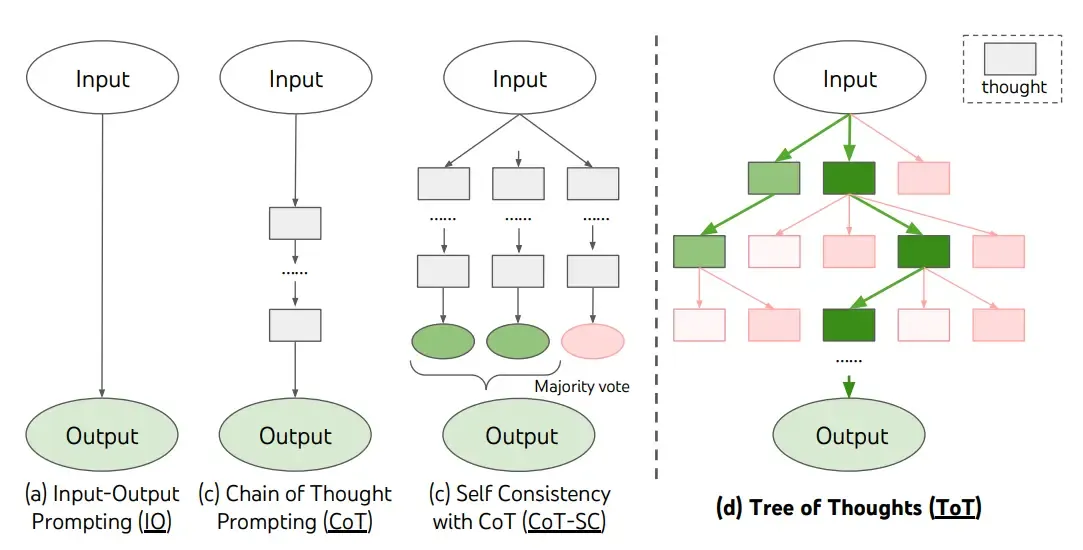
\includegraphics[width=\textwidth,height=0.8\textheight,keepaspectratio]{images/lrm+moe/reasoning-techniques.png}
        \caption*{Input-output prompting, Chain-of-Thought, Self-Consistency and Tree-of-Thought side by side. Source: \href{https://arxiv.org/abs/2305.10601}{Yao et al. (2023)}, Fig.~1.}
    \end{figure}
\end{frame}

\subsection{Chain-of-Thought (CoT) Prompting}
\begin{frame}{Chain-of-Thought Prompting (Recap)}
    \begin{itemize}
        \item CoT prompting makes the model generate intermediate reasoning steps before the final answer, either by showing worked examples or by appending ``Let's think step by step''.
        \item For reasoning models this is the central mechanism: the techniques that follow make the intermediate steps longer, broader, or trained into the weights.
        \item Beyond basic CoT: automatic exemplar construction (Auto-CoT), search over reasoning paths (Tree-of-Thought), and sampling-based answer selection (Self-Consistency).
    \end{itemize}
\end{frame}

\begin{frame}{Few-shot vs Zero-shot CoT}
    \begin{itemize}
        \item Few-shot CoT provides worked exemplars in the prompt (e.g. ``If 6 times 4 equals 24, then what is 6 times 5?'' followed by its reasoning steps); zero-shot CoT only appends an instruction such as ``Let's think step by step''.
        \item Few-shot buys accuracy at the cost of hand-crafting exemplars for each task; zero-shot avoids that cost but is weaker on hard problems. Auto-CoT aims for few-shot accuracy without the manual effort.
    \end{itemize}
    \begin{figure}[h]
        \centering
        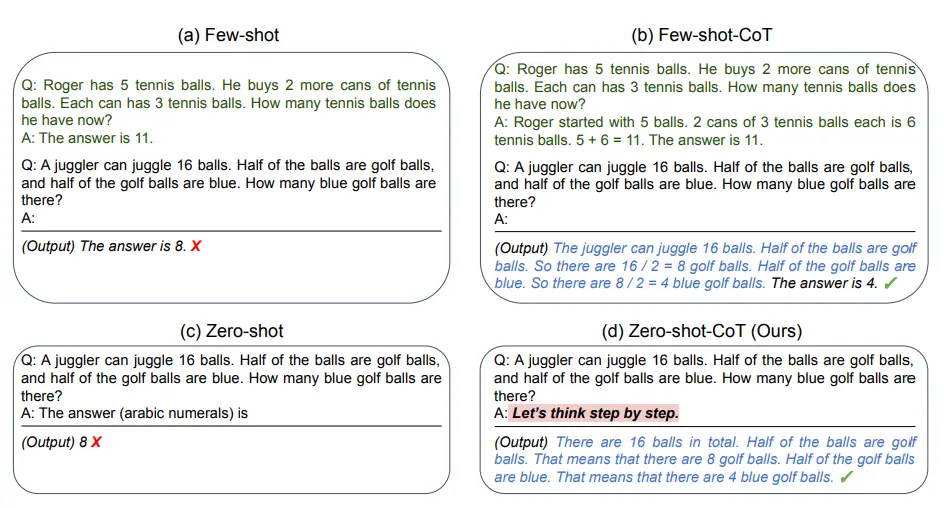
\includegraphics[height=0.34\textheight,width=\textwidth,keepaspectratio]{images/lrm+moe/few-shot_zero-shot.png}
        \caption*{Four prompting settings on the same question: (a) Few-shot, (b) Few-shot-CoT, (c) Zero-shot and (d) Zero-shot-CoT. Only the two CoT settings reach the right answer. Source: \href{https://arxiv.org/abs/2205.11916}{Kojima et al. (2022)}, Fig.~1.}
    \end{figure}
\end{frame}


\begin{frame}[allowframebreaks]{Auto-CoT Prompting}
    \begin{figure}[h]
        \centering
        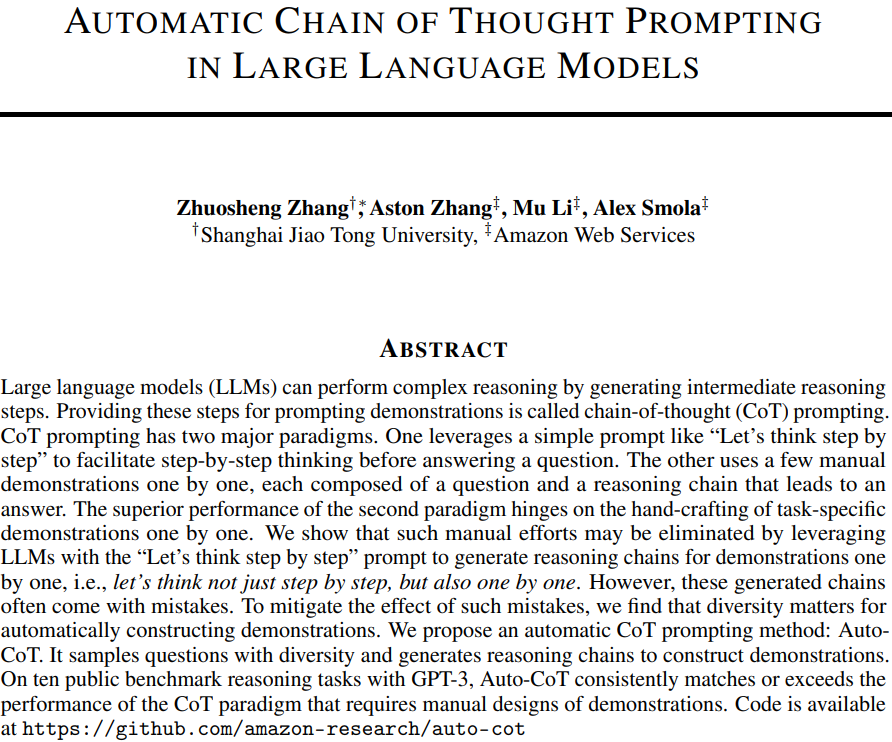
\includegraphics[height=0.9\textheight,width=\textwidth,keepaspectratio]{images/lrm+moe/paper-auto-cot.png}
    \end{figure}
    \begin{itemize}
        \item \textbf{What is Auto-CoT?}
        \begin{itemize}
            \item A method for building the worked exemplars that few-shot CoT needs, without writing them by hand.
            \item The reasoning chains in the prompt are generated by the model itself rather than by an annotator.
        \end{itemize}
        \item \textbf{How it works:}
        \begin{itemize}
            \item \textbf{Cluster:} encode the task's questions with Sentence-BERT and partition them into $k$ clusters.
            \item \textbf{Construct:} from each cluster take the question closest to the centre and generate its chain with Zero-shot CoT (``Let's think step by step''), keeping the first chain that passes simple length and format criteria.
            \item The $k$ resulting question-and-chain pairs become the few-shot prompt. Clustering spreads the exemplars over different question types, so one flawed chain cannot dominate the prompt.
        \end{itemize}
    \framebreak
        \item \textbf{Benefits:}
        \begin{itemize}
            \item Removes the manual effort of writing exemplars while matching, and on some benchmarks exceeding, hand-crafted few-shot CoT.
            \item Needs only a pool of unlabelled questions from the task: no reference reasoning chains and no answer labels.
        \end{itemize}
        \item \textbf{Cost:}
        \begin{itemize}
            \item The exemplars are only as good as the zero-shot chains behind them, so the selection criteria are what keep wrong reasoning out of the prompt.
        \end{itemize}
    \end{itemize}
    \framebreak
    \begin{figure}[h]
        \centering
        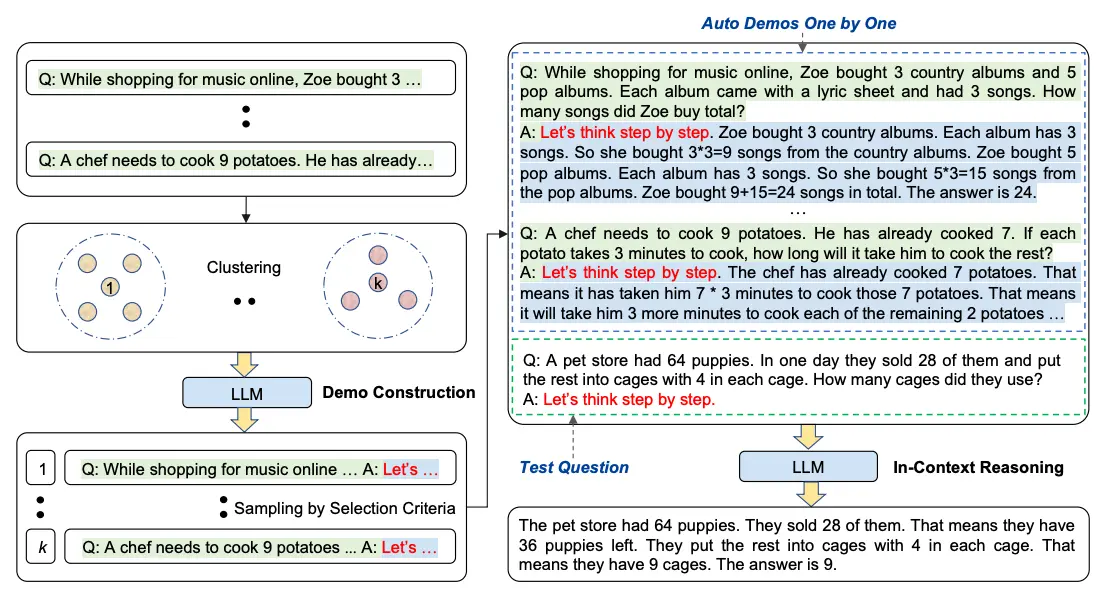
\includegraphics[height=0.8\textheight,width=\textwidth,keepaspectratio]{images/lrm+moe/auto-cot.png}
        \caption*{Auto-CoT Prompting. Source: \href{https://arxiv.org/abs/2210.03493}{Zhang et al. (2022)}, Fig.~4.}
    \end{figure}
    \framebreak
    \begin{figure}[h]
        \centering
        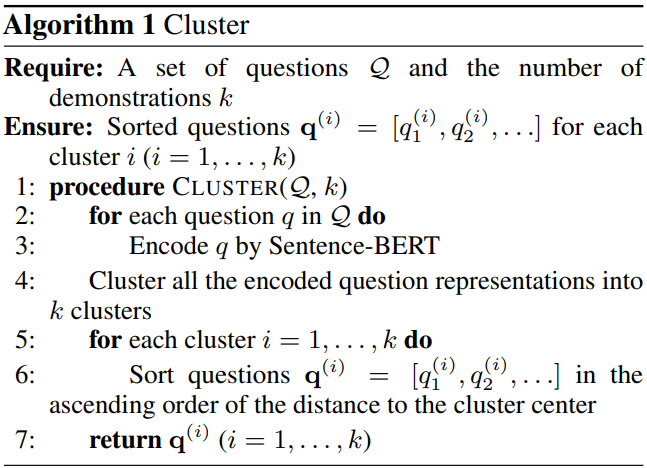
\includegraphics[height=0.8\textheight,width=\textwidth,keepaspectratio]{images/lrm+moe/algo-auto-cot-cluster.png}
        \caption*{Clustering step: group the task's questions and sort each cluster by distance to its centre. Source: \href{https://arxiv.org/abs/2210.03493}{Zhang et al. (2022)}, Alg.~1.}
    \end{figure}
    \framebreak
    \begin{figure}[h]
        \centering
        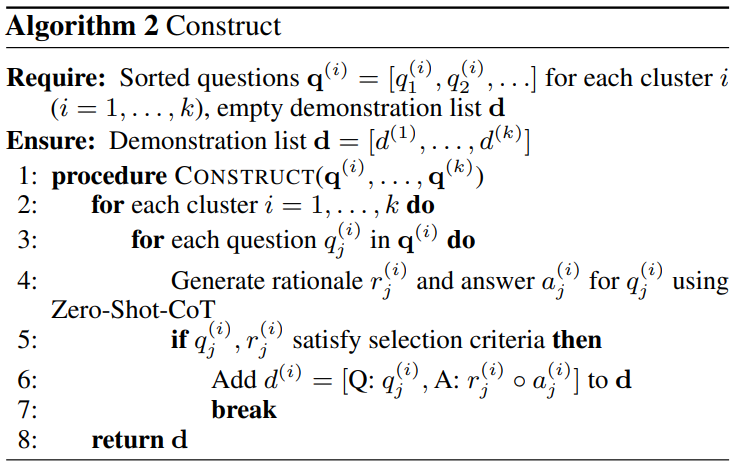
\includegraphics[height=0.72\textheight,width=\textwidth,keepaspectratio]{images/lrm+moe/algo-auto-cot-construct.png}
        \caption*{Construction step: generate a chain per cluster with Zero-shot CoT and keep the first that passes the selection criteria. Source: \href{https://arxiv.org/abs/2210.03493}{Zhang et al. (2022)}, Alg.~2.}
    \end{figure}
\end{frame}


\subsection{Tree-of-Thought (ToT) Reasoning}
\begin{frame}[allowframebreaks]{Tree-of-Thought (ToT) Reasoning}
    \begin{figure}[h]
        \centering
        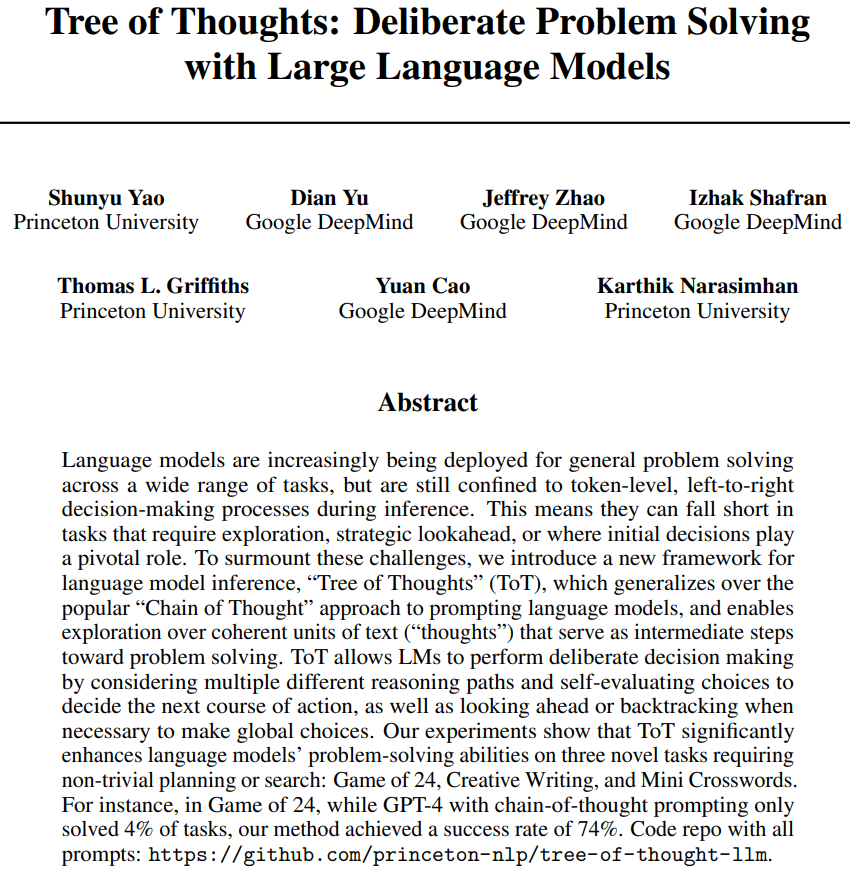
\includegraphics[height=0.9\textheight,width=\textwidth,keepaspectratio]{images/lrm+moe/paper-tot.png}
    \end{figure}
    \begin{itemize}
        \item \textbf{What is ToT?}
        \begin{itemize}
            \item A reasoning technique that structures the thought process as a tree, allowing for exploration of multiple reasoning paths.
            \item Each node in the tree represents a step in the reasoning process, and branches represent different possible paths or decisions.
        \end{itemize}
        \item \textbf{How it works:}
        \begin{itemize}
            \item The model generates a tree structure where each branch represents a different reasoning path.
            \item The model can explore multiple paths simultaneously, evaluating the outcomes of each.
        \end{itemize}
    \framebreak
        \item \textbf{Benefits:}
        \begin{itemize}
            \item Allows for more complex reasoning by considering multiple possibilities at once.
            \item Helps the model avoid getting stuck in a single line of reasoning, improving problem-solving capabilities.
        \end{itemize}
        \item \textbf{Example (Game of 24):}
        \begin{itemize}
            \item Given four numbers, reach 24 using each exactly once. A thought is one intermediate equation, e.g.\ ``$4 + 9 = 13$ (left: 5, 10, 13)''.
            \item At each level the model proposes candidate next equations, then rates each resulting state as sure, maybe, or impossible, and only the most promising states are expanded.
            \item Search matters here because a single greedy chain commits to its first arithmetic step and cannot recover: CoT solves 4\% of these puzzles, ToT with breadth 5 solves 74\%.
        \end{itemize}
    \end{itemize}
    \framebreak
    \begin{figure}[h]
        \centering
        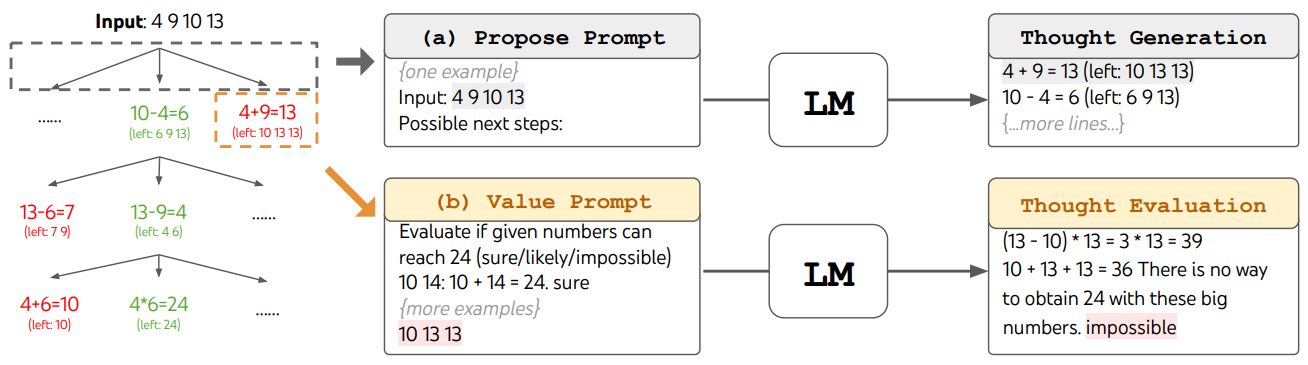
\includegraphics[height=0.8\textheight,width=\textwidth,keepaspectratio]{images/lrm+moe/tot-reasoning.png}
        \caption*{ToT in a game of 24. The LM is prompted for (a) thought generation and (b) valuation. Source: \href{https://arxiv.org/abs/2305.10601}{Yao et al. (2023)}, Fig.~2.}
    \end{figure}
    \framebreak
    \begin{figure}[h]
        \centering
        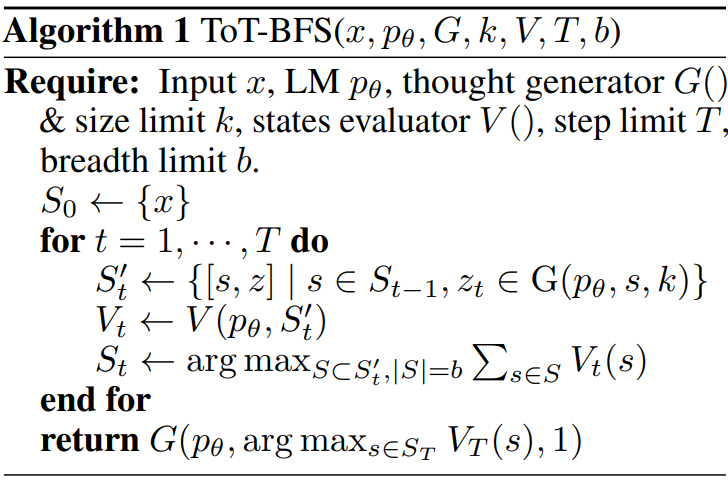
\includegraphics[height=0.8\textheight,width=\textwidth,keepaspectratio]{images/lrm+moe/algo-tot-bfs.png}
        \caption*{Breadth-first search over thoughts: keep the $b$ best-valued states at each of the $T$ levels. Source: \href{https://arxiv.org/abs/2305.10601}{Yao et al. (2023)}, Alg.~1.}
    \end{figure}
    \framebreak
    \begin{figure}[h]
        \centering
        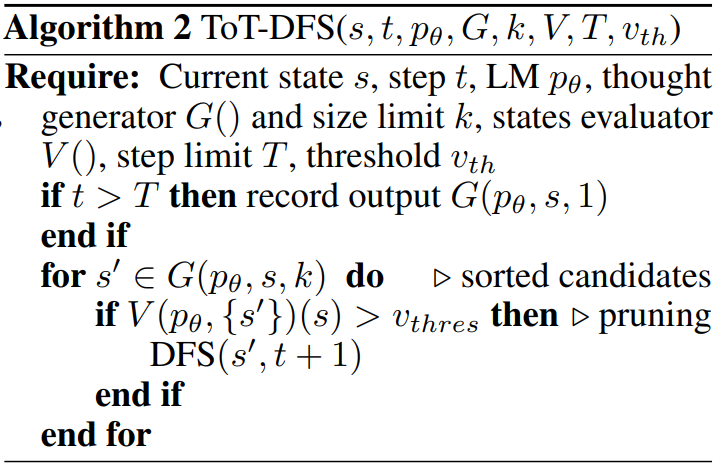
\includegraphics[height=0.8\textheight,width=\textwidth,keepaspectratio]{images/lrm+moe/algo-tot-dfs.png}
        \caption*{Depth-first search over thoughts: follow one branch, pruning any state valued below the threshold $v_{th}$. Source: \href{https://arxiv.org/abs/2305.10601}{Yao et al. (2023)}, Alg.~2.}
    \end{figure}
    \framebreak
    \begin{figure}[h]
        \centering
        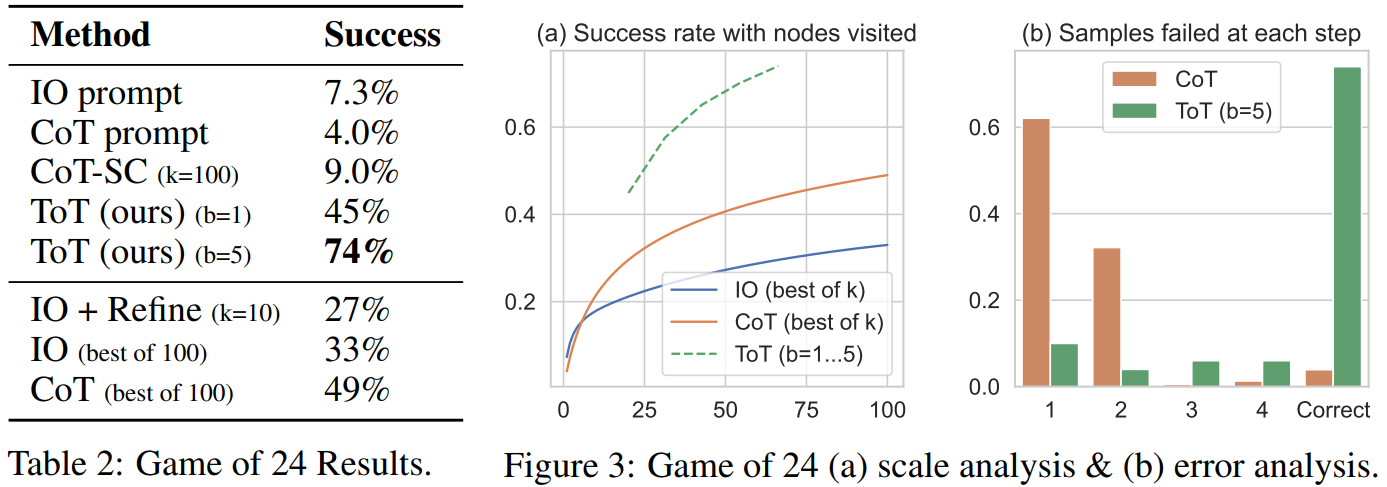
\includegraphics[height=0.8\textheight,width=\textwidth,keepaspectratio]{images/lrm+moe/tot-analysis+result.png}
        \caption*{Source: \href{https://arxiv.org/abs/2305.10601}{Yao et al. (2023)}, Table~2 and Fig.~3.}
    \end{figure}
    \framebreak
    \begin{figure}[h]
        \centering
        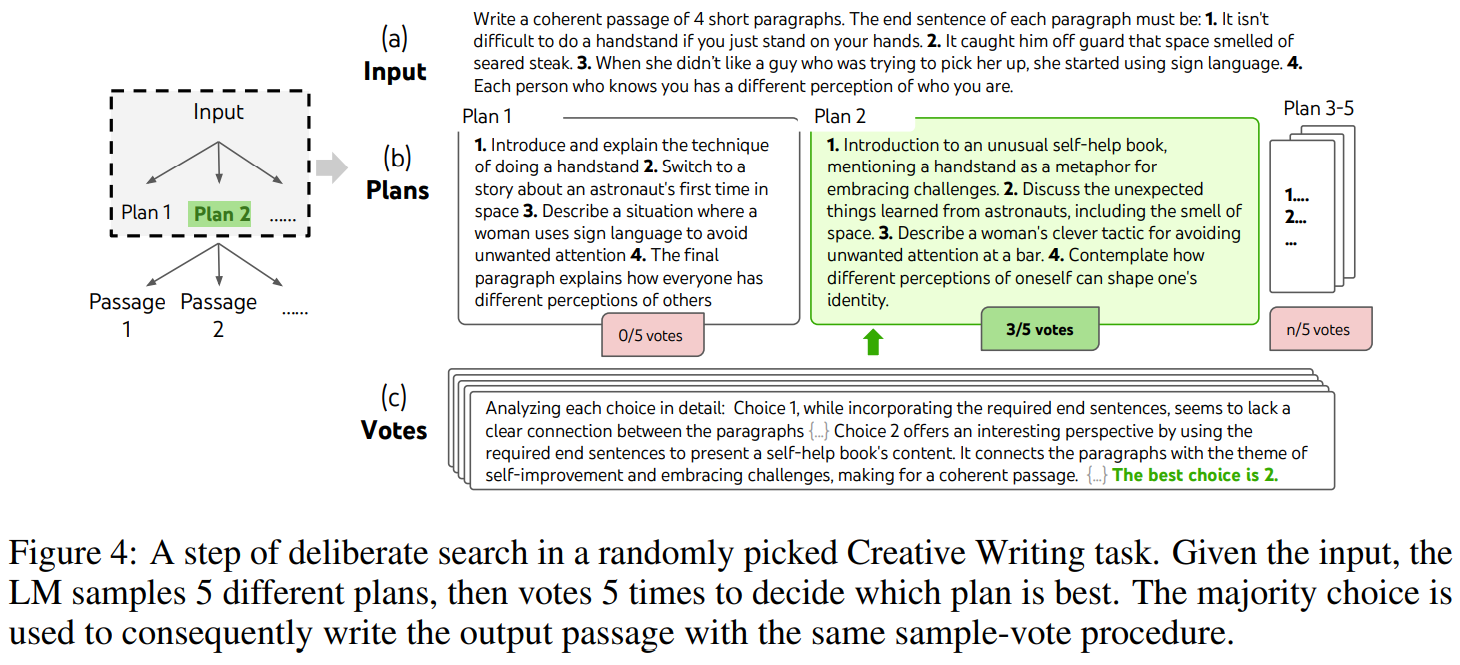
\includegraphics[height=0.8\textheight,width=\textwidth,keepaspectratio]{images/lrm+moe/tot-creative-writing-task.png}
        \caption*{Source: \href{https://arxiv.org/abs/2305.10601}{Yao et al. (2023)}, Fig.~4.}
    \end{figure}
    \framebreak
    \begin{figure}[h]
        \centering
        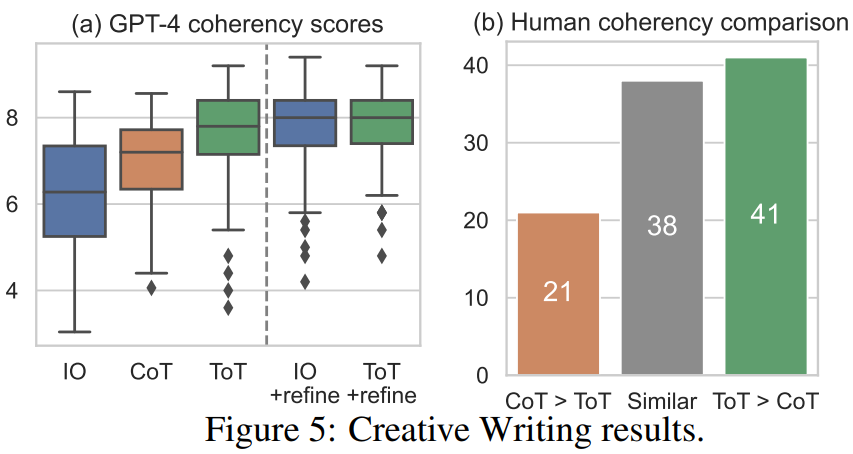
\includegraphics[height=0.8\textheight,width=\textwidth,keepaspectratio]{images/lrm+moe/tot-creative-writing-result.png}
        \caption*{Source: \href{https://arxiv.org/abs/2305.10601}{Yao et al. (2023)}, Fig.~5.}
    \end{figure}
\end{frame}


\subsection{Self-Consistency (SC)}
\begin{frame}[allowframebreaks]{Self-Consistency (SC)}
    \begin{itemize}
        \item Self-consistency samples several reasoning paths for the same prompt, then keeps the answer the paths agree on.
        \item The figures below give the empirical picture from Wang et al. (2022): consistent gains across arithmetic and commonsense benchmarks, growing with the number of sampled paths, at a linear increase in inference cost.
        \item Sampling many paths at inference time is an early form of test-time compute scaling, the same trade later used by dedicated reasoning models.
    \end{itemize}
    \framebreak
    \begin{figure}[h]
        \centering
        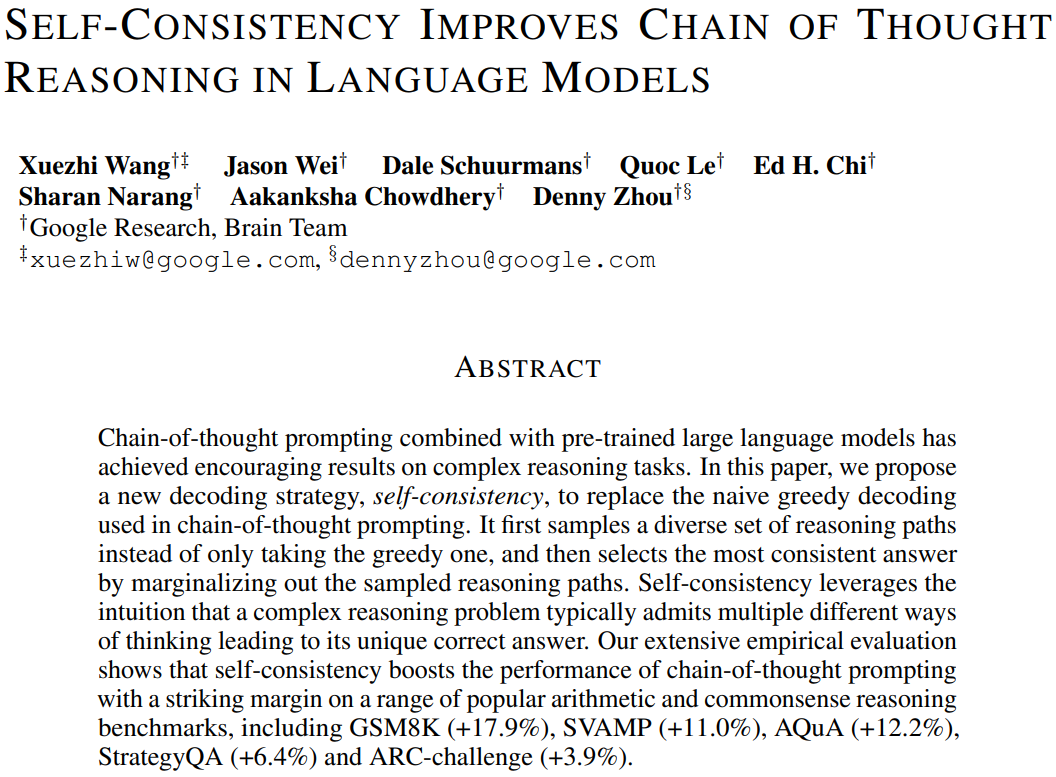
\includegraphics[height=0.9\textheight,width=\textwidth,keepaspectratio]{images/lrm+moe/paper-self-consistency.png}
    \end{figure}
    \framebreak
    \begin{figure}[h]
        \centering
        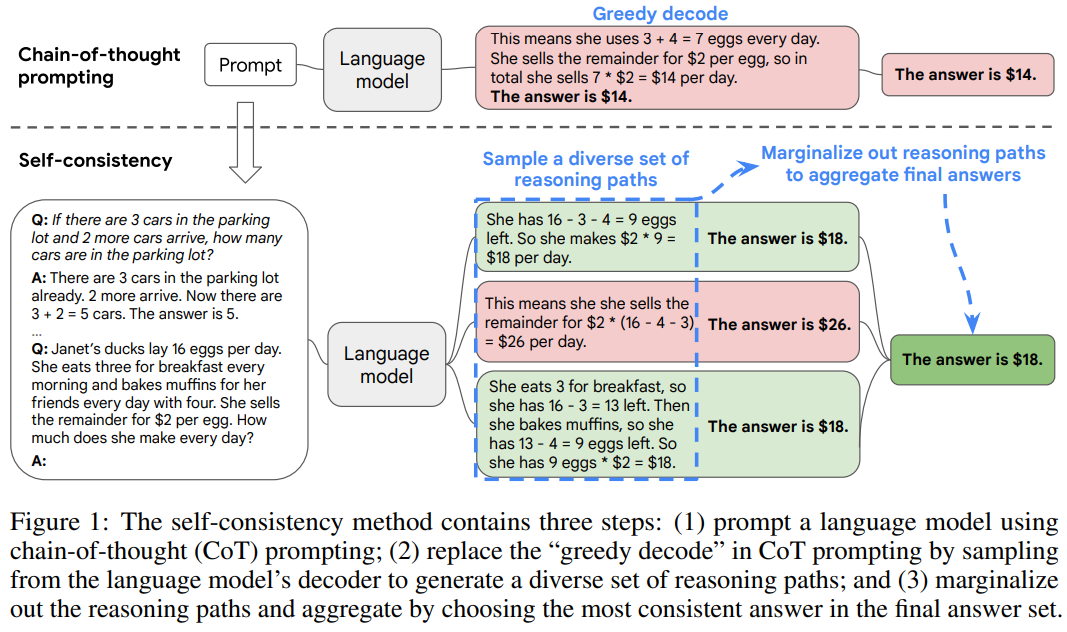
\includegraphics[height=0.8\textheight,width=\textwidth,keepaspectratio]{images/lrm+moe/self-consistency.png}
        \caption*{Source: \href{https://arxiv.org/abs/2203.11171}{Wang et al. (2022)}, Fig.~1.}
    \end{figure}
    \framebreak
    \begin{figure}[h]
        \centering
        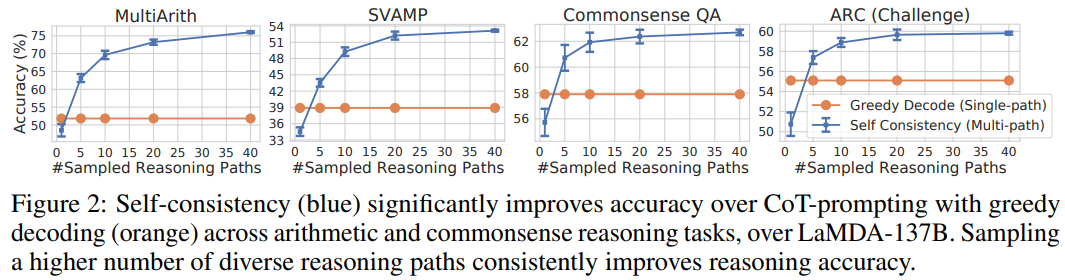
\includegraphics[height=0.8\textheight,width=\textwidth,keepaspectratio]{images/lrm+moe/self-consistency-accuracy.png}
        \caption*{Source: \href{https://arxiv.org/abs/2203.11171}{Wang et al. (2022)}, Fig.~2. Note that the gain saturates: extra samples buy less and less.}
    \end{figure}
    \framebreak
    \begin{figure}[h]
        \centering
        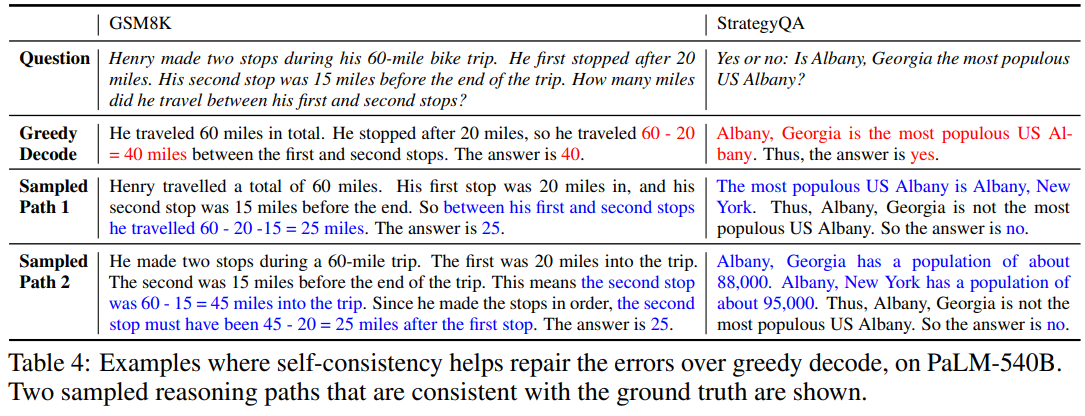
\includegraphics[height=0.8\textheight,width=\textwidth,keepaspectratio]{images/lrm+moe/self-consistency-benchmark.png}
        \caption*{Source: \href{https://arxiv.org/abs/2203.11171}{Wang et al. (2022)}, Table~4.}
    \end{figure}
    \framebreak
    \begin{figure}[h]
        \centering
        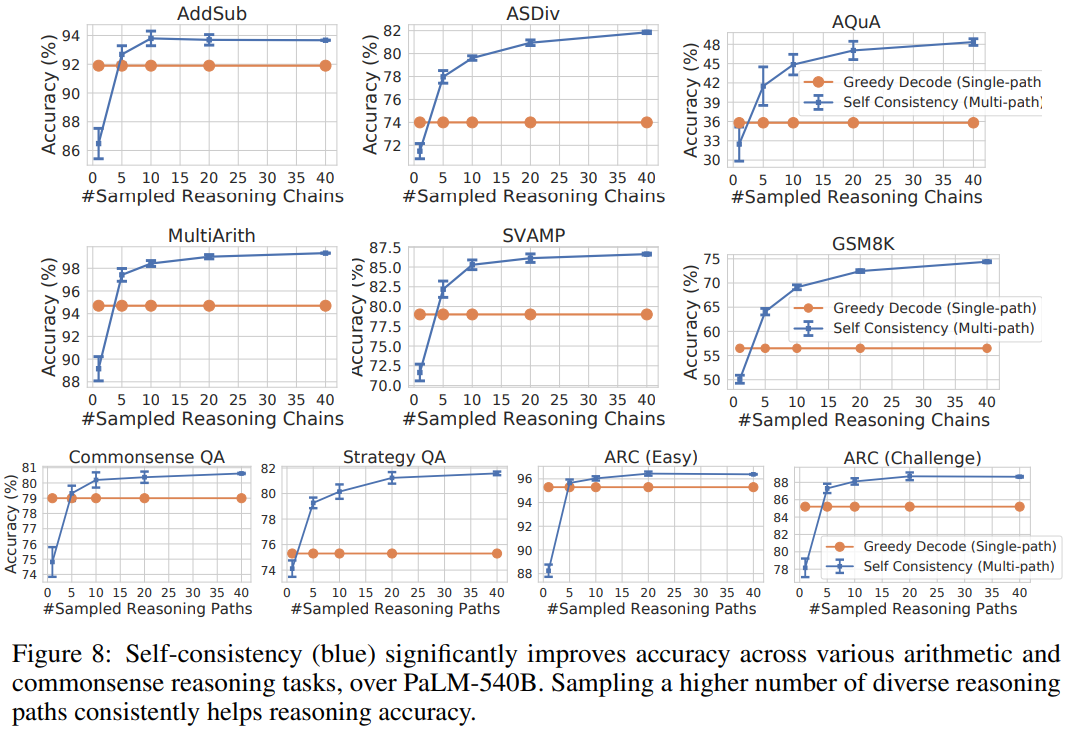
\includegraphics[height=0.72\textheight,width=\textwidth,keepaspectratio]{images/lrm+moe/self-consistency-accuracy-2.png}
        \caption*{Source: \href{https://arxiv.org/abs/2203.11171}{Wang et al. (2022)}, Fig.~8.}
    \end{figure}
\end{frame}